\documentclass[11pt]{article}

\usepackage{pdflscape}
\usepackage{graphicx}
\usepackage[hidelinks]{hyperref}

\begin{document}

\begin{titlepage}
	\begin{center}
		
		\begin{figure}[t]
			\centering
			
\includegraphics[width=350px]{../Images/UP_Logo.png}
		\end{figure}
		
		% Title
		\textsc{\large } \\ 
		\vspace{2cm}
		\textbf{\Huge IMY 310 Project  \\
			Project Plan \\
			(Phase 1)} \\ 

		\textsc{\large } \\ 
		\vspace{0.75cm}

		\textbf{\Large AgriSales Magazine} \\ 
		
		\begin{flushright} \large
			Azhar Mohungoo \emph{12239799} \newline
			Daniel Malangu \emph{} \newline
			Kudzai  	\emph{} \newline
			\newline
			Group Name  \emph{} \newline
			\end{flushright}
		%\end{minipage}
		
	\end{center}
\end{titlepage}


\tableofcontents

\listoffigures

\newpage

\section{Paper Prototype Designs}
	
	\subsection{Original Designs}
	
	\subsubsection{Home Page}
		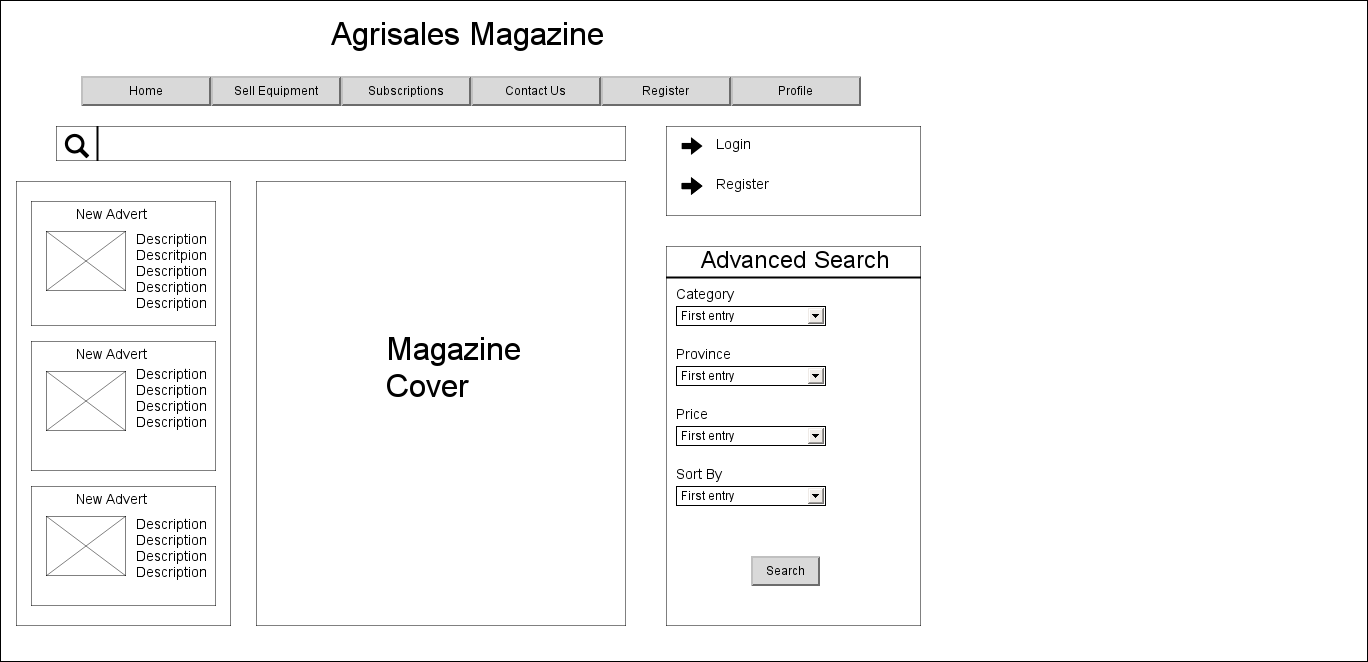
\includegraphics[width=0.75\linewidth]{../Images/Agrisales-HomePage}
		
	\subsubsection{Login Page}
		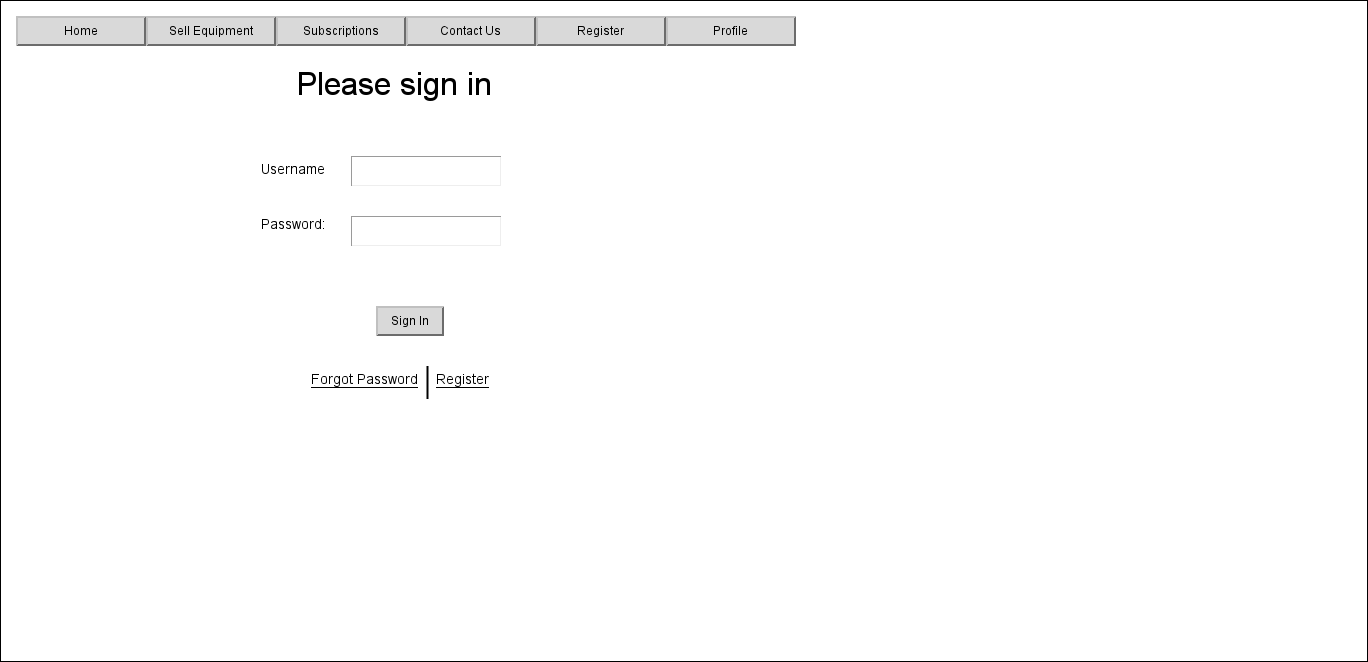
\includegraphics[width=0.75\linewidth]{../Images/Agrisales-LoginPage}
		
	\subsubsection{Registration Page}
		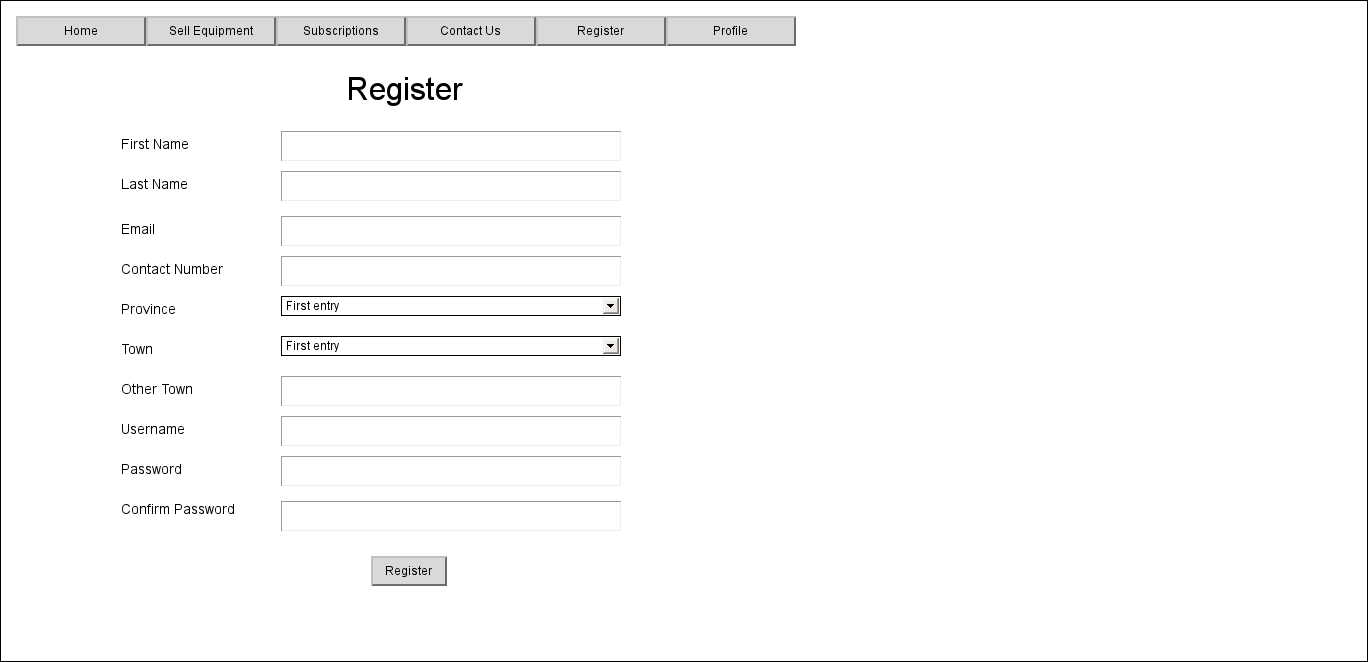
\includegraphics[width=0.75\linewidth]{../Images/Agrisales-RegistrationPage}
		
	\subsubsection{Advertisements Page}
		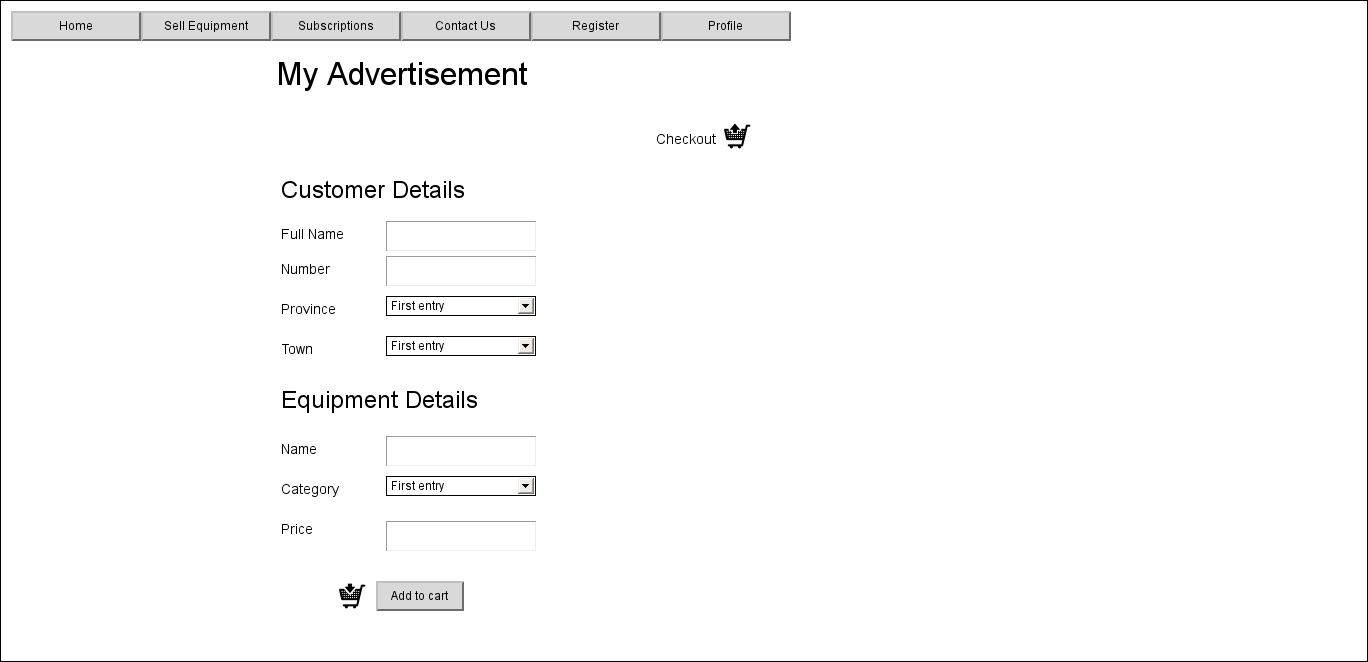
\includegraphics[width=0.75\linewidth]{../Images/Agrisales-AdvertisementsPage}
		
	\subsubsection{Subscriptions Page}
		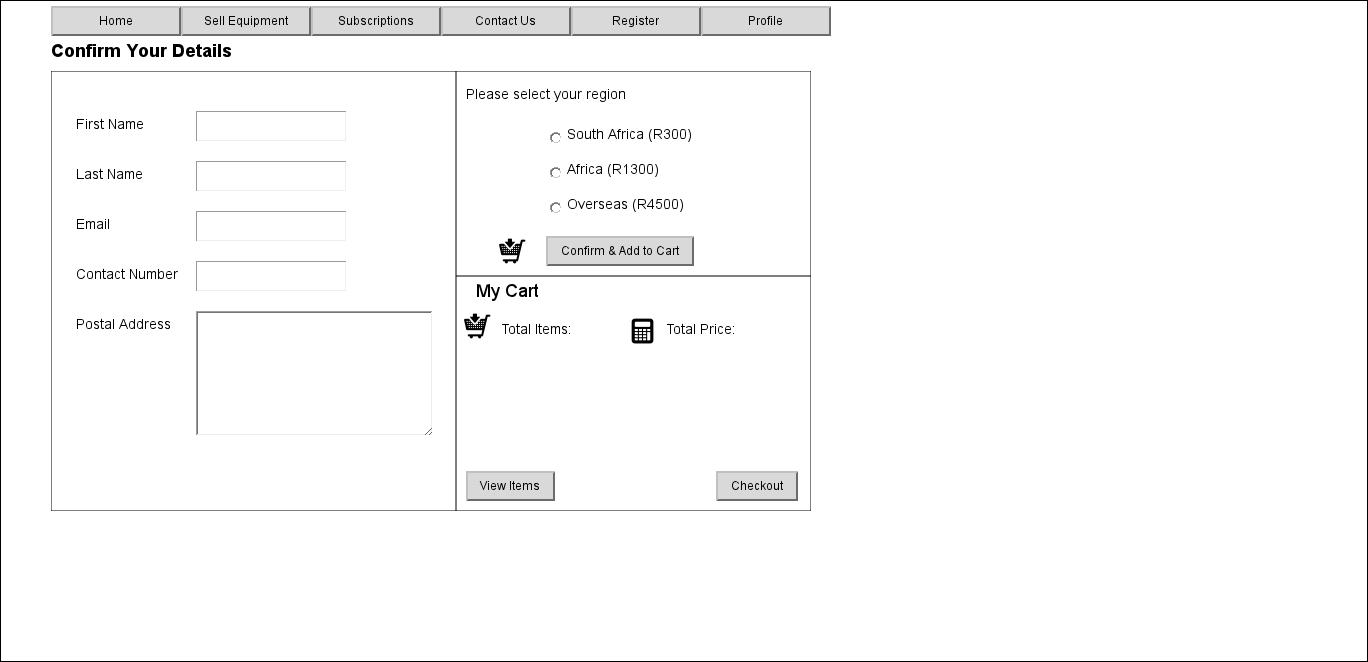
\includegraphics[width=0.75\linewidth]{../Images/AgriSales-SubscriptionsPage}
		
	\subsubsection{View Ad Page}
		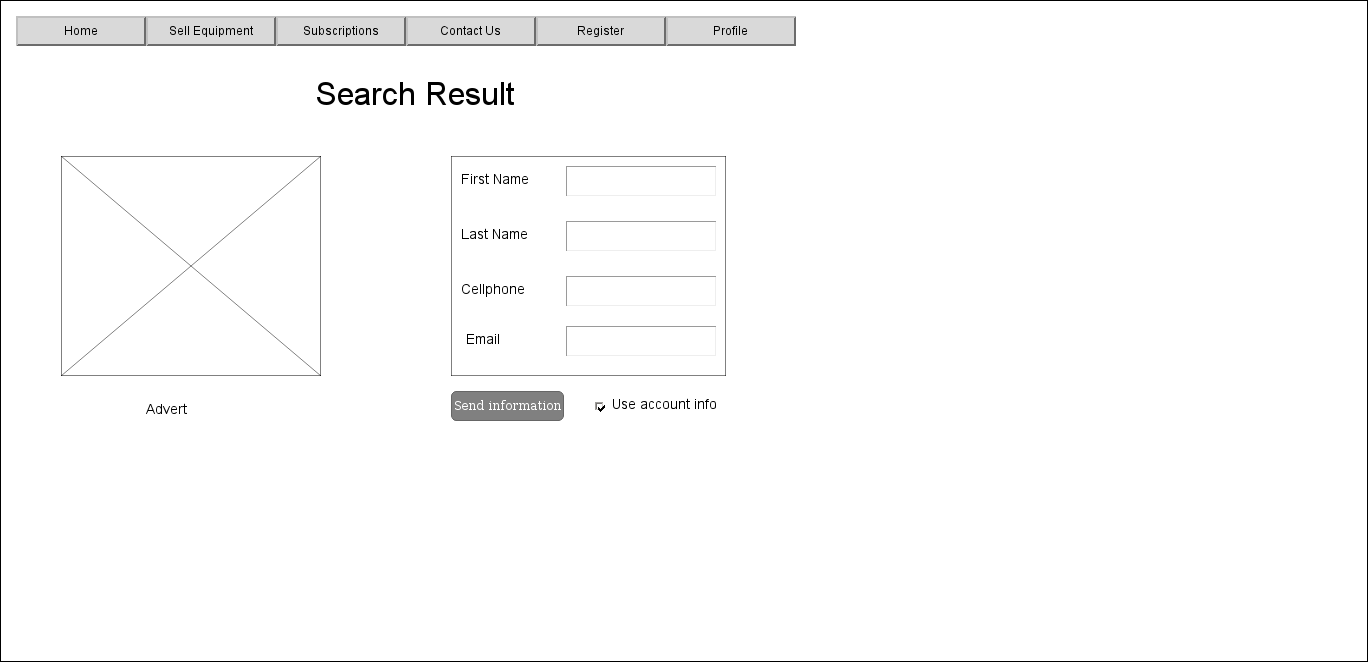
\includegraphics[width=0.75\linewidth]{../Images/AgriSales-ViewAdPage}
		
	\subsubsection{Contact Us Page}
		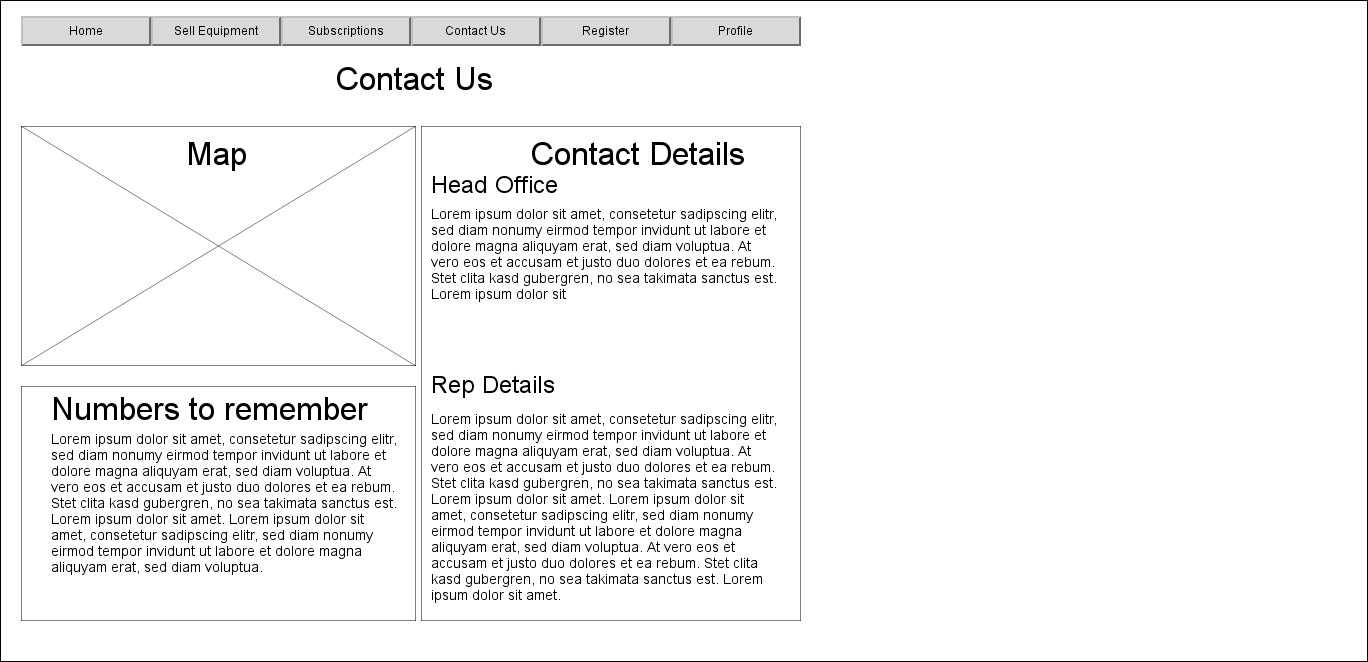
\includegraphics[width=0.75\linewidth]{../Images/Agrisales-ContactUsPage}
		
	\subsubsection{Alternative Home Page}
		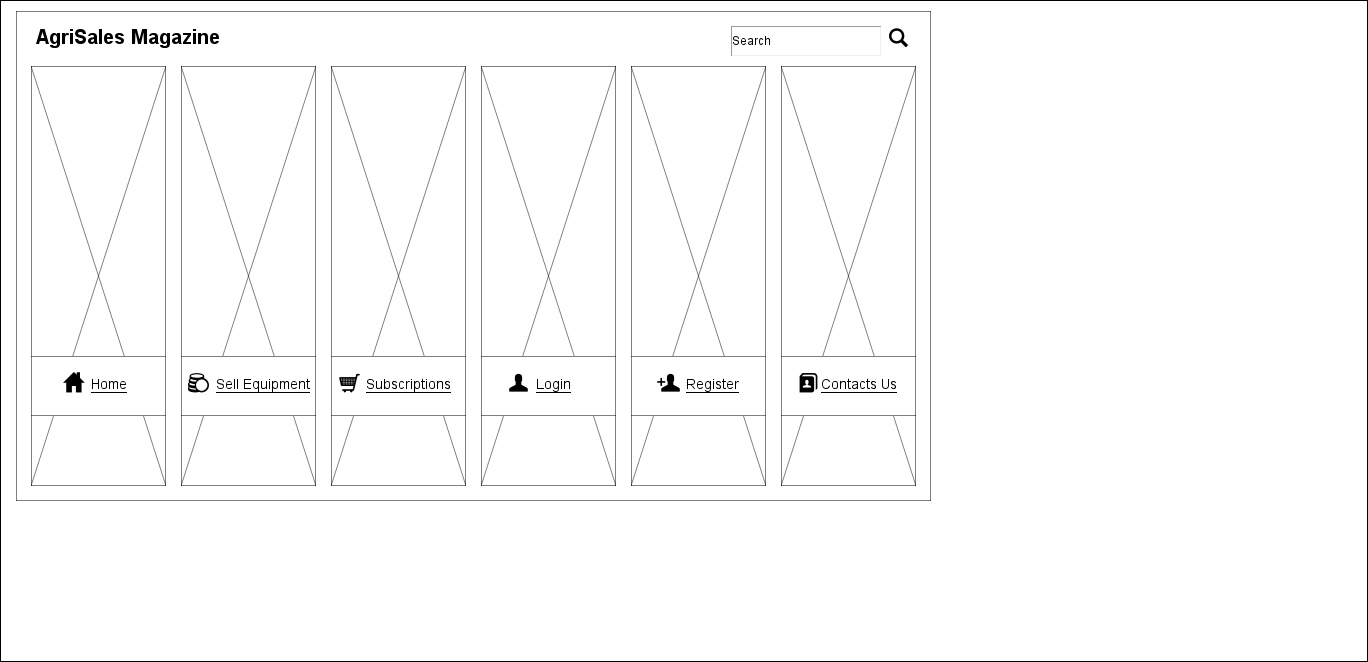
\includegraphics[width=0.75\linewidth]{../Images/AgriSales-AlternativeHomePage}
		
	\subsubsection{Alternative Advertisement Page}
		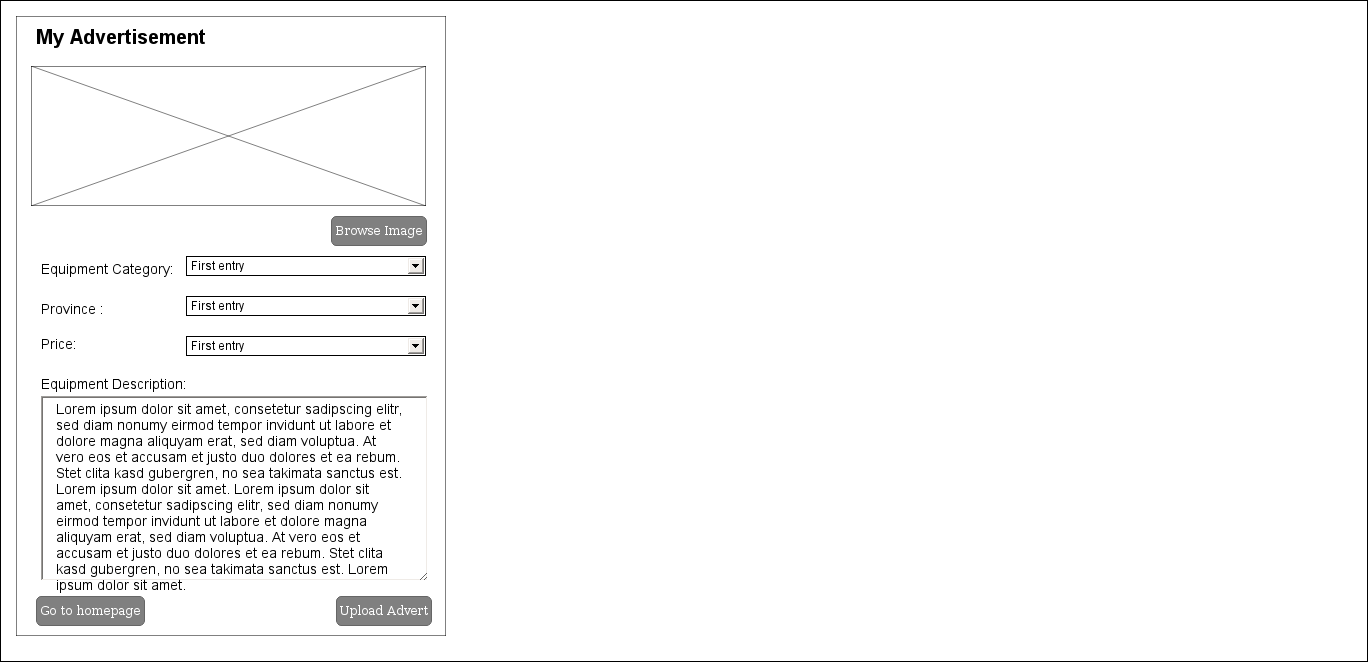
\includegraphics[width=0.75\linewidth]{../Images/AgriSales-AlternativeAdvertisementPage}
		
	\subsubsection{Alternative Subscriptions Page}
		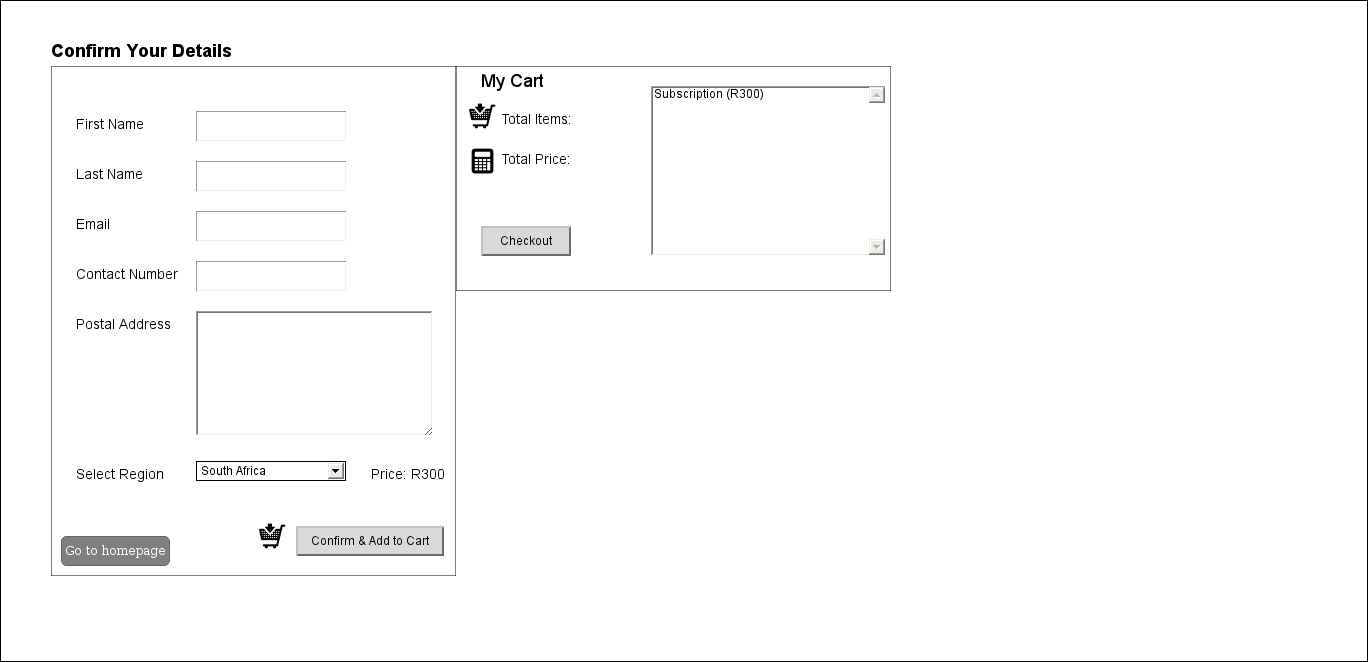
\includegraphics[width=0.75\linewidth]{../Images/AgriSales-AlternativeSubscriptionsPage}
		
	\subsubsection{Alternative Contact Us Page}
		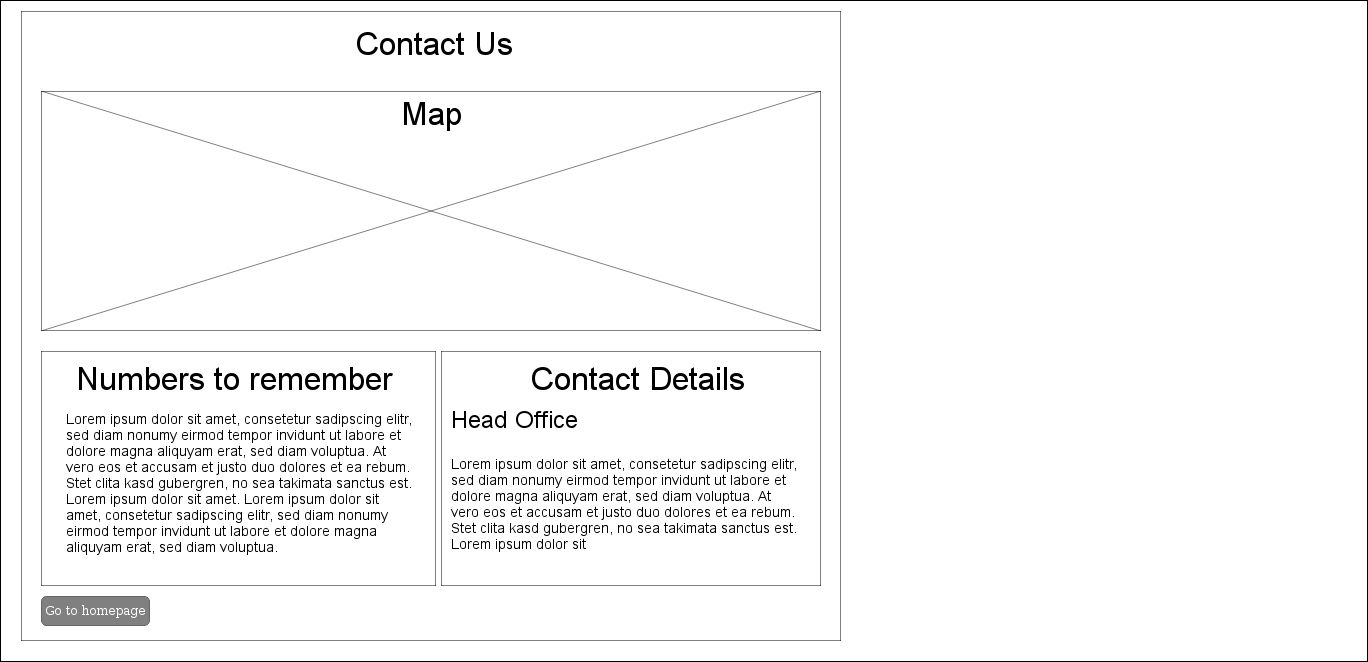
\includegraphics[width=0.75\linewidth]{../Images/AgriSale-AlternativeContactUsPage}

\newpage

\section{Motivations for Alternative Designs}
	The reasoning behind the first design was to have the functionality for the website easily available to the users. Our users would not have to traverse the site too many times to find what they are looking for, whether they are searching for equipment to buy or whether they want to sell their own equipment, because the home page leads to most, if not all, of the desired functionality. \\
	
	The motivation for the second design was to make the website as clear and as simple as possible. The design is meant to make it easy for the user to find what they are looking for by not cluttering the pages with too much information and by providing clearly labeled links to the website pages. Traversing through the website may take longer in this design, however, it has less chance of having the user being lost or not finding what they are looking for.

\section{Testing the Designs}
	When testing, we presented our paper based designs to the stakeholders in a sequential order starting from the home page. We proceeded to each of the options within the menu of the home page, while providing them with explanations on how the product functions moving from one web page to the other. 
	
	\begin{center}
		\begin{tabular}{ |p{3cm}||p{10cm}| } 
			\hline
			Sell Equipment &  It takes you to the sell equipment page where you	 will be able to upload an image and details of a piece of equipment that you would like to get rid of. In order to be able to do this  action you need to be logged in \\ 
			\hline
			Subscriptions &  It allows you to subsribe to the magazine\\ 
			\hline
			Contact Us & It takes you to a page which provides the user with information about the locations and contact details of offices \\ 
			\hline
			Login & Allows a user to login to the website. You need to be registered to do this \\ 
			\hline
			Register & Allows a user to register to the website inorder to allow the user to subscribe and use other functions \\ 
			\hline
			Profile & View your own profile, but you need to be logged in to view it \\
			\hline
		\end{tabular} 
	\end{center}
	
	The stakeholders then provided us with comments about the sketches, which in turn helps us determine what they expect and what changes they would like to make for the product.

\section{Feedback Received}
	The design of our paper based prototypes was shown to a sample of our stakeholders so their input could be used to generate a product design to meet their requirements.
	\begin{itemize}
		\item A few were concerned about the lack of colours in the paper prototypes.
		\item The layout of the main page was mostly mentioned as an impressive part of the design
		\item Functionality was said to be clearly visible in terms of the required information to be given to a function
		\item Alternative design of the pages were favoured a bit more due to the layout having less options
		\item The floating menu bar is out of place on some pages
		\item Some of the functionality requires for a lot of fields to be filled
	\end{itemize}
\section{Using the Feedback}
	The user feedback is an important tool in the design phase when making a product. This is how we plan on using it to better satisfy the requirements set by ourstakeholders
	\begin{itemize}
		\item Keep the labeling on the pages short and using more icons so functionality can be understood without having to read too much	
		\item Reduce the functionality to require more clicking of buttons than the filling of forms
		\item Changing the menu bar to better suit the layout
	\end{itemize}
\end{document}
